In this section, we explore how nature can ``trick'' us when we wield the
\textit{tools of god}---namely, polynomials---to fit our models to data.
Polynomial regression is still a linear regression model (linear in the
parameters), but by expanding the feature space with polynomial terms we can
capture much more \textit{sensual}, non-linear structures in $x$.

\vspace{0.2cm}

This apparent power comes with a catch: high-degree polynomials are so
flexible that they can bend to pass through almost every training point,
including noise, without actually capturing the underlying structure we care
about. In other words, complexity can become our downfall: more degrees do not
always mean better generalization. (Moral: do not be a greedy sonnovabitch!)

\subsection*{Polynomial regression}
Polynomial regression is an instance of linear regression:
\[
Y = w_0 + w_1 X + w_2 X^2 + \cdots + w_p X^p + \varepsilon,
\]
where
\[
\min_{w}\;\frac{1}{2n}\sum_{i=1}^n \Big( y_i - (w_0 + w_1 x_i + w_2 x_i^2 + \cdots + w_p x_i^p) \Big)^2,
\]
with $\operatorname{deg}(Y) = p = M$.

\medskip

\noindent We present some examples for these type of regressions and choose different \textit{degrees} for our polynomial in order to see explicitly the trickery we've discussed.
\begin{itemize}
    \item $M=0,1,3,9$
\end{itemize}

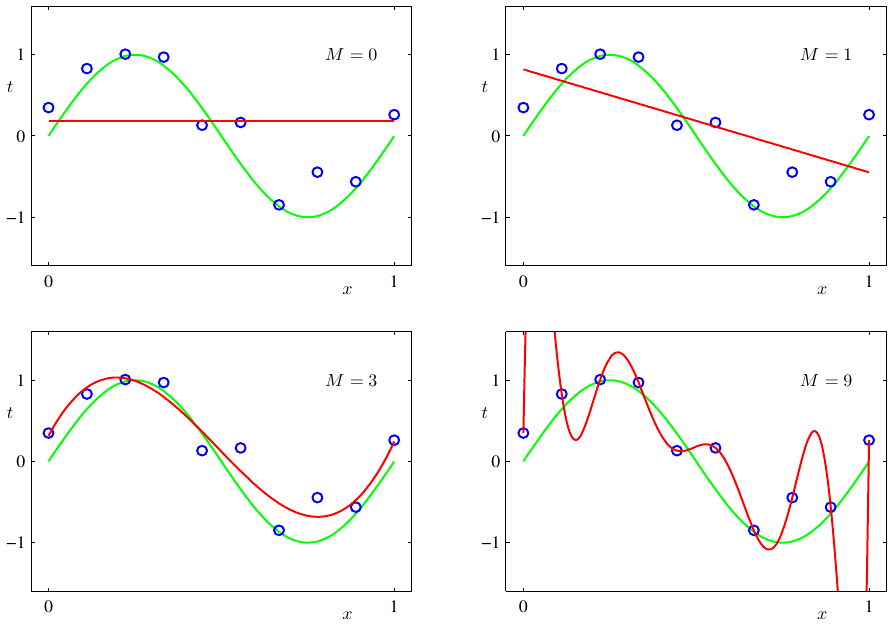
\includegraphics[width=0.8\textwidth]{figures/poly_regression_examples.png}

\subsection*{Overfitting: symptoms and characteristics}
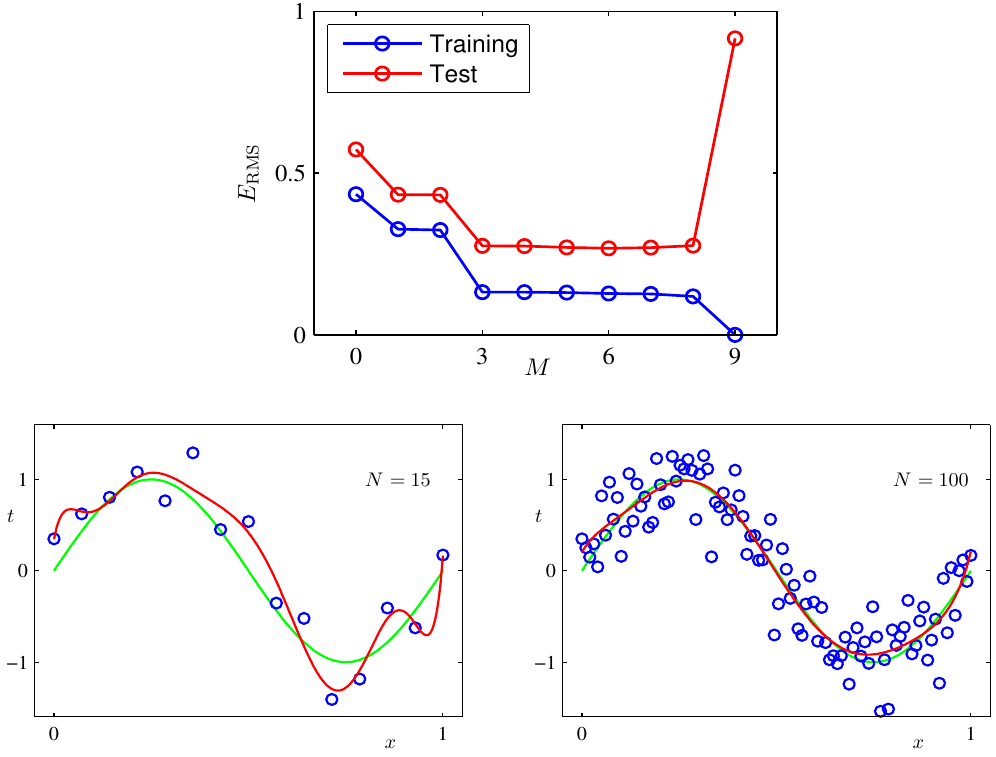
\includegraphics[width=0.8\textwidth]{figures/overfitting_training_test.png}

This trickery we've talked about is formally known as \textit{overfitting}. Most of the times, it posseses some of the characteristics we descibe below (which are clearly visible from our figures above).
\begin{itemize}
    \item Training error decreasing \textit{monotonically} (i.e. consistently decreasing) as complexity increases.
    \item Test error decreasing initially, then increasing as the model begins to fit noise.
\end{itemize}

\subsection*{Overfitting and generalization}
In machine learning/statistics, the main concern is the \emph{generalization ability} of the predictor.

\medskip

\noindent Fitting the data perfectly does \emph{not always} mean poor generalization.  
For example: deep neural networks in computer vision often fit perfectly and still generalize well.

\medskip

\noindent However, fitting perfectly \emph{is problematic} if:
\begin{itemize}
    \item The data is noisy and the model fits the noise.
    \item The model must become overly complex in order to fit the data.
\end{itemize}

\medskip

So, we confront a big and intimidating wall which may as well be reduced if we're able to answer the following question: How do we measure \textbf{complexity}?

\subsection*{Tikhonov regularization}
Courtesy of Andrey N. Tikhonov (1906--1993).

\medskip

\noindent Regularized Empirical Risk Minimization (ERM) objective:
\[
\min_{f \in S} \; \hat R_n(f) + \lambda \|f\|^2,
\]
where $\lambda$ is the \textit{regularization} coefficient or \textit{hyperparameter}.

\medskip

\begin{proposition} How to know if the above objective is well posed?
    \begin{itemize}
        \item If $\hat R_n$ is convex:
        \begin{enumerate} 
            \item $\implies$ objective is strongly convex and coercive for any $\lambda > 0$.
            \item $\implies$ solution exists and is unique.
            \item $\implies \text{  }\lambda \mapsto \hat f_\lambda$ is a continuous function.
        \end{enumerate}
        \item If $\hat R_n$ is only bounded below:
        \begin{enumerate}
            \item $\implies$ objective is coercive and at least one solution exists.
        \end{enumerate}
        \item If $\hat R_n$ is $C^2$ with bounded curvature:
        \begin{enumerate}
            \item $\implies$ regularization eliminates small local minima.
        \end{enumerate}
    \end{itemize}
\end{proposition}

Well, since that is a mouthfull, let us digress with an insightfull remark.

\begin{remark}[Strong convexity and coercivity]
Let $f:\mathbb{R}^d \to \mathbb{R}$ be differentiable.
\begin{itemize}
  \item \textbf{Convex:} $f$ is convex if for all $x,y\in\mathbb{R}^d$ and $t\in[0,1]$,
  \[
  f(tx+(1-t)y) \;\leq\; t f(x) + (1-t)f(y).
  \]

  \item \textbf{Strongly convex:} $f$ is $\mu$-\emph{strongly convex} ($\mu>0$) if
  \[
  f(y) \;\geq\; f(x) + \nabla f(x)^\top (y-x) + \frac{\mu}{2}\|y-x\|^2
  \quad \forall x,y\in\mathbb{R}^d.
  \]
  Intuitively, the graph of $f$ always curves upwards at least as much as a quadratic bowl of curvature $\mu$.
  Strong convexity implies that the minimizer of $f$ is \emph{unique}.

  \item \textbf{Coercive:} $f$ is coercive if
  \[
  \|x\| \to \infty \;\;\;\implies\;\;\; f(x) \to +\infty.
  \]
  This condition ensures that a minimizer cannot ``escape to infinity'',
  so a minimizer exists (at least one).
\end{itemize}

\noindent
\emph{In ridge regression:} the regularized risk
\[
\hat R_n(w) + \frac{\lambda}{2}\|w\|^2
\]
is $\lambda$-strongly convex and coercive for any $\lambda>0$,
hence it always admits a unique solution.
\end{remark}


\subsection*{Ridge regression}
Applying Tikhonov regularization to OLS:
\[
\min_{w\in\mathbb{R}^p} \frac{1}{2n}\|y - Xw\|_2^2 + \frac{\lambda}{2}\|w\|_2^2.
\]

Normal equations:
\[
\Big(\tfrac{1}{n}X^\top X + \lambda I\Big)w = \tfrac{1}{n}X^\top y,
\]
so the unique solution is:
\[
\hat w_{\text{ridge}} = \frac{1}{n}\Big(\tfrac{1}{n}X^\top X + \lambda I\Big)^{-1}X^\top y.
\]

\begin{remark}[Normal equations]
In ordinary least squares we minimize
\[
\min_{w \in \mathbb{R}^p} \; \|y - Xw\|_2^2.
\]
Setting the gradient to zero yields
\[
X^\top X w = X^\top y,
\]
a system of linear equations called the \emph{normal equations}.
They are called ``normal'' because the residual vector
$r = y - X\hat w$ is orthogonal (normal) to the column space of $X$,
\textbf{not} because of any assumption about normally distributed noise.
\end{remark}


\subsection*{Linear vs affine regression and regularization}
\[
f_w(x) = w^\top x
\quad\text{vs}\quad
f_{w,b}(x) = w^\top x + b = \tilde w^\top \tilde x,
\]
with
\[
\tilde w = \begin{bmatrix} w \\ b \end{bmatrix}, \qquad 
\tilde x = \begin{bmatrix} x \\ 1 \end{bmatrix}.
\]

Thus, an affine model in dimension $p$ is a linear model in dimension $p+1$.

\medskip

\noindent Difference: When regularizing, usually $b$ is not penalized.  
So minimizing
\[
\min_{w\in\mathbb{R}^p} \frac{1}{2n}\|y - Xw + b1\|_2^2 + \frac{\lambda}{2}\|w\|_2^2
\]
is not equivalent to penalizing $\tilde w$.

\subsection*{Polynomial regression with ridge}
We now explore an example of polynomial regression for the parameters $n=10$, degree $M=9$ (look how different the behaviour is from not regularizing!). We also compare
 no regularization with that of ridge regularization for different values of $\lambda$.

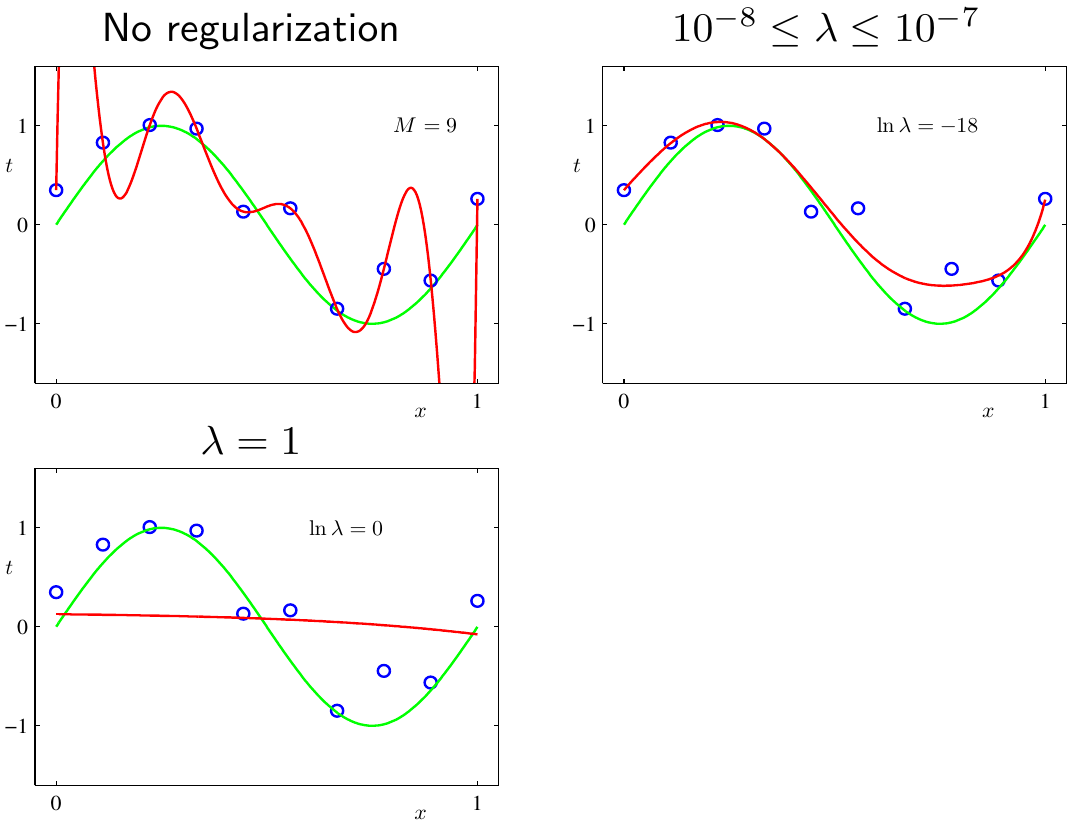
\includegraphics[width=0.8\textwidth]{figures/poly_ridge_examples.png}

Also, note the difference between our train v. test error evolution with and without regularization. It is now more stable for greater degrees of the polynomial.

\vspace{0.2cm}

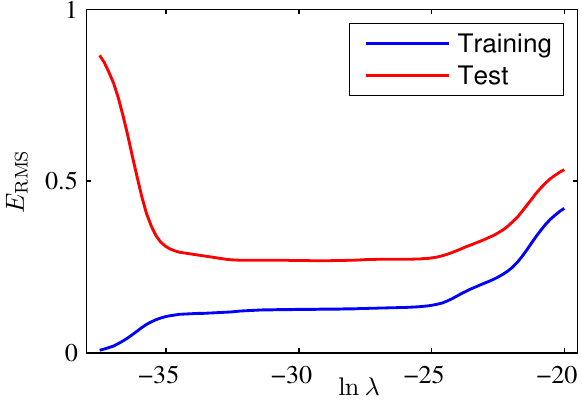
\includegraphics[width=0.8\textwidth]{figures/poly_ridge_err.png}


\subsection*{Controlling complexity of the hypothesis space}
Explicit control:
\begin{itemize}
    \item number of variables,
    \item max polynomial degree,
    \item spline degree and number of knots,
    \item max resolution in wavelet approximation,
    \item bandwidth in RKHS.
\end{itemize}

Implicit control:
\begin{itemize}
    \item via regularization,
    \item Bayesian formulations,
    \item optimization algorithm itself,
    \item randomization, etc.
\end{itemize}

\medskip

\noindent The complexity of the predictor often results from a trade-off between goodness of fit and complexity.  
\textbf{Model selection problem:} how to choose the right level of complexity?

\subsection*{Risk decomposition: approximation--estimation trade-off}
Let $f^*$ be the target function, $f^*_S = \arg\min_{f\in S} R(f)$, and $\hat f_S$ the ERM predictor in $S$.

\[
R(\hat f_S) - R(f^*) \;=\;
\underbrace{R(\hat f_S) - R(f^*_S)}_{\text{estimation error}}
+ \underbrace{R(f^*_S) - R(f^*)}_{\text{approximation error}}.
\]

This is sometimes called the \emph{bias--variance trade-off}.

\subsection*{Approximation--estimation trade-off}
There is generally a compromise:
\begin{itemize}
    \item fitting the training data well,
    \item avoiding a too complex model to ensure generalization.
\end{itemize}

\noindent However, this view has been challenged by modern neural networks.